
\documentclass[12pt,letterpaper]{article}
%\documentclass[final]{siamltex}
\usepackage[top=1.0in,left=1.0in,footskip=0.75in,marginparwidth=1in]{geometry}
\usepackage{epstopdf}
\usepackage{amsmath,amssymb,amsbsy,graphics,graphicx,setspace,float,enumitem,bm,mathabx,mathrsfs}
\usepackage{indentfirst,verbatim}
\usepackage{subfig,booktabs}

\def\vecsign{\mathchar"017E}
\def\dvecsign{\smash{\stackon[-1.95pt]{\vecsign}{\rotatebox{180}{$\vecsign$}}}}
\def\dvec#1{\def\useanchorwidth{T}\stackon[-4.2pt]{#1}{\,\dvecsign}}
\usepackage{stackengine}
\stackMath

% use Unicode characters - try changing the option if you run into troubles with special characters (e.g. umlauts)
\usepackage[utf8]{inputenc}

% clean citations
\usepackage{cite}

% hyperref makes references clicky. use \url{www.example.com} or \href{www.example.com}{description} to add a clicky url
\usepackage{nameref,hyperref}

% improves typesetting in LaTeX
\usepackage{microtype}

% text layout - change as needed
\raggedright
\setlength{\parindent}{0.75cm}
\textwidth 6.50in
\textheight 8.75in

\newcommand{\natwidthpng}{610}
\newcommand{\natheightpng}{642}

% use adjustwidth environment to exceed text width (see examples in text)
\usepackage{changepage}

% adjust caption style
\usepackage[aboveskip=1pt,labelfont=bf,labelsep=period,singlelinecheck=off]{caption}
\captionsetup{justification=centering}

% headrule, footrule and page numbers
\usepackage{lastpage,fancyhdr,graphicx}
\usepackage{epstopdf}
\pagestyle{myheadings}
\pagestyle{fancy}
\fancyhf{}
\rfoot{\thepage/\pageref{LastPage}}
\renewcommand{\footrule}{\hrule height 2pt \vspace{2mm}}
\fancyheadoffset[R]{0.0in}
\fancyfootoffset[R]{0.0in}

% use \textcolor{color}{text} for colored text (e.g. highlight to-do areas)
\usepackage{color}

% define custom colors (this one is for figure captions)
\definecolor{Gray}{gray}{.25}

% this is required to include graphics
\usepackage{graphicx}

% use if you want to put caption to the side of the figure - see example in text
\usepackage{sidecap}

% document begins here
\begin{document}
\vspace*{0.35in}

% title goes here:
\begin{centering}
{
\Large
\textbf{MUI Coupling Tutorial in AMReX} \\
\large
\textbf{Exchanging data between two executables} \\
}

\end{centering}

\section*{Goal}

\noindent The goal of this tutorial is to incorporate the MxUI/MUI (Multiscale Universal Interface) framework into AMReX. This framework allows two separate executables to communicate with one another in parallel using MPI. In addition, this framework is adaptable for different geometries, in which the bounds of data one would like to send and/or receive can be specified using the {\fontfamily{qcr}\selectfont announce\_send\_span()} and {\fontfamily{qcr}\selectfont announce\_recv\_span()} commands.

\section*{Operation \& Test Case}

\noindent In this tutorial, two different C++ codes are built separately. Each has different spatial dimensions: one is built in 3D ({\fontfamily{qcr}\selectfont AMREX\_SPACEDIM = 3}), and the other in 2D ({\fontfamily{qcr}\selectfont AMREX\_SPACEDIM = 2}). Each code is compiled separately within their respective ``exec'' directories {\fontfamily{qcr}\selectfont Exec\_01 \& Exec\_02}, after which the two executables are run together using the following command, specifying the number of MPI processes to designate to each executable:

\begin{verbatim}
$ mpirun -np N1 ../Exec_01/main3d.gnu.MPI.ex inputs
: -np n2 ../Exec_02/main2d.gnu.MPI.ex inputs
\end{verbatim}

\noindent on a single line within the {\fontfamily{qcr}\selectfont Exec\_coupled} directory. {\fontfamily{qcr}\selectfont N1} and {\fontfamily{qcr}\selectfont n2} are the number of MPI ranks designated for each executable, respectively. Each executable is given the same inputs file within {\fontfamily{qcr}\selectfont Exec\_coupled}. Input variables {\fontfamily{qcr}\selectfont max\_grid\_size\_3d} and {\fontfamily{qcr}\selectfont max\_grid\_size\_2d} determine the respective grid sizes for 3D and 2D. As far as I am aware, the code works for any AMReX grid structure. Details of how to build and run the code are contained in the script {\fontfamily{qcr}\selectfont cmd\_mpirun}.\\

\vspace{0.5cm}
\noindent Figure 1 shows one possible grid structure of the 2D (red grid) and 3D (multicolored blocks) setup.

\begin{figure}[H]
    \centering
    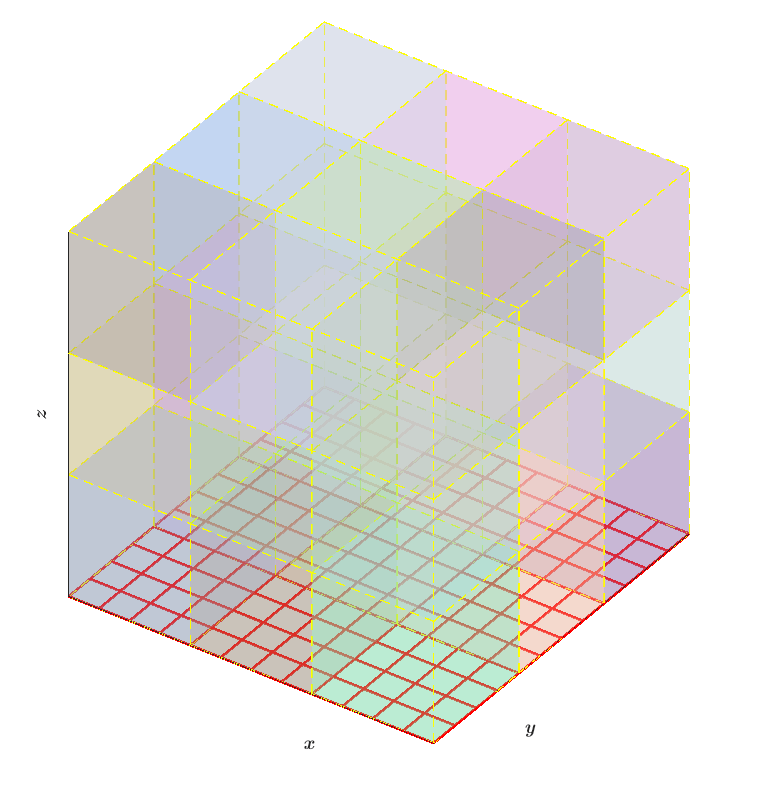
\includegraphics[width=0.80\textwidth,natwidth=\natwidthpng,natheight=\natheightpng]{iface_rect.png}
    \caption{3D and 2D grid setup - rectangular 2D grids}
\end{figure}

\vspace{0.5cm}
\noindent The 3D code initializes a 3D MultiFab (Note: with no ghost cells), and sends a 2D slice of this data at the $k = 0$ location to the 2D executable, which stores the data in a 2D MultiFab, multiplies the data by a constant, and sends the modified platter back to the 3D executable. Finally, the 3D executable receives the modified data and places it back into the 3D MultiFab, at $k = 0$. \\

\vspace{0.5cm}
\noindent The 2D, original 3D, and modified 3D data are all written to separate plot files, which can be visualized using software such as Amrvis. \\

\section*{Additional Comments}

\vspace{0.5cm}
\noindent Although our code does not include this, it would be possible to pair an AMReX code with code that is outside of the AMReX framework, because each code is compiled separately. For example, using the {\fontfamily{qcr}\selectfont announce\_send\_span()} and {\fontfamily{qcr}\selectfont announce\_recv\_span()} commands, MUI would be able to determine the overlap between the two regions to correctly exchange the data, even if the two grid structures differ.

\end{document}

